
\part*{Conclusion} % 16p
\addcontentsline{toc}{part}{Conclusion}
%\chaptermark{Conclusion}



% Purvis: God, I'm so tired.
% Johner: Sleep when you die, man.


\begin{comment}
* Discussion, future work and conclusion - 16p
** Discussion - 3p
** Future work for Cheops - 10p
*** Ownership Types - 4p
*** Classification - 4p
*** Other collaborations - 2p
** Conclusion - 3p
\end{comment}

\epigraph{\emph{Christie:} How many [..] are there?\\
\emph{Dr. Wren:} Twelve.}{\emph{Alien: Resurrection}}


\chapter{Discussion} % 3p
%\addcontentsline{toc}{chapter}{Discussion}
\label{chap:discussion}

This chapter is dedicated to discussions around the approach, its
inherent limitations and what could be done better or in the future.
%
There is an entire chapter (\autoref{chap:future-work}) for the
perspectives on the approach, but in this chapter, we will only talk
about small changes that could be done in the Cheops implementation
and would not fundamentally change the approach.

The first small point to discuss is the naming ``service mesh'' itself.
%
The approach is called service mesh because of the definition of
William Morgan~\autoref{chap:soa-SM} (page~\pageref{chap:soa-SM}).
%
It is a layer handling service-to-service communication that delivers
request through the topology of services of cloud native applications,
implemented as an array of proxy alongside the services, and the
application is not aware.
%
In Cheops, the only functionality is to help the application running
at the Edge by managing the geo-distribution of instances of this
application.
%
But Cheops also fulfills some of the functionalities of an API
gateway, if we consider this definition from IBM~\cite{api-gateway}:
%
\begin{quote}
  \emph{An application programming interface (API) gateway is software
    that takes an application user’s request, routes it to one or more
    backend services, gathers the appropriate data and delivers it to
    the user in a single, combined package. It also provides
    analytics, layers of threat protection and other security for the
    application.}

  \emph{An API gateway provides a single entry point for all API calls that
  come into an application, whether the app is hosted in an
  on-premises data center or on the cloud. It accepts requests that
  come in remotely and returns the requested data.}
\end{quote}
The functionalities of analytics, threat protection and security are
definitely not considered, but what is done is Cheops could be viewed
as a decentralized API gateway (with several entry points that are
only the same Cheops instantiated on every site).
%
Overall, the name ``service mesh'' has been chosen to help grasping
the idea of what we do more easily, but we have functionalities from
different ways to manage services from Cloud applications.


Our approach, as it as been said, takes into account different
interesting features or way to approach problems that have been presented
in the state-of-the-art, ~\autoref{p:soa}.
%
The closest approach is~\cite{MWY+17}, which uses some kind of sharing
collaboration for Glance, tracks ID of the resources, and has
autonomous instances of \os on each site.
%
Cheops differs mainly by being more generic and using different types
of collaboration to fulfill the single coherent view.


\section{Application version}

As discussed before in~\autoref{sec:principles}, the approach
relies on the modularity of service-based Cloud applications, so it is
not viable for any type of Cloud applications.
%
It requires microservices-based applications that exposes an API for
services communications.
%
These applications also need to be able to work on a single site since
they will deployed autonomously on every sites.
%
Moreover, it has been mentioned shortly, but every instance of the
services should have the same version so they have identical models of
their resources and they have the same API.

%
This can be restrictive as it is difficult for different actors on the
entire infrastructure to maintain the same version, as it has been
seen with \os, different businesses often have their own version of
the application and have different versions of the application, some
dating from several years; and it is actually the case sometimes in
the same actor with different
locations\footnote{\url{https://cleura.com/services/cloud-features/regions-and-services/}
  - Accessed 2022-10-12}.
%
This is mainly because it is difficult to update a running
application, but also because it is difficult for open-source
applications to be tailored for every use case possible.


\section{Consistency}

\subsection{Consistency from the API}

This approach ensures consistency at the service-level, but for the
resources they manage.
%
The only operations available to manipulate these resources are
therefore the ones exposed by the API.
%
Thus, the resources are maintained as identical as the API allows it,
but nothing more and any change on the resources that can be done
internally make the replicas diverge from others.
%
For example, in the \os case, VMs created through replication will
have the same specifications, but everything done internally on the
VMs will not be replicated to other VMs as the application API does
not allow to make these changes.

It is a limitation of the approach, but this consistency \emph{inside}
the resources is not desired as it requires to know the internals of
the application and reproduce it outside or add code inside the
application to provide an API.
%
% For example, nothing can be said about the consistency of two VMs
% booted through this process; their internal state will probably
% diverge, as expected.

\subsection{Better consistency}

Raft is a distributed consensus algorithm using an elected leader to
apply the changes made on replicas.
%
The leader sends changes to the followers and await confirmation of
the majority of followers to confirm the change before committing it.
%
In our case, since we cannot always assume it is possible to rollback
a change in a resource, we only ensure that a majority of nodes are
available before sending the request to be executed.
%
Thus, the consistency is only ensured eventually, when the changes
will be executed on all involved replicas.

% en fait ça sera ptêtre meme pas le cas mdr (si site revient pas)
As another consensus algorithm, Epaxos could be considered, to avoid
designated leaders~\cite{MAK13, TPO21}.
%
% Epaxos

The use of Conflict-free Replicated Data Types (CRDT)~\cite{PBS18,
  SPBZ11} is also currently under study for future versions of Cheops.


\section{What can be improved in Cheops}

First of all, it is important to mention once again
(see~\autoref{sec:validation}) that in our current implementation of
Cheops, in order to simplify the process, we decided to avoid the
interception part as it is mostly technical.
%
Nonetheless, it should be considered for the validity of
the approach as it could be a problem for some applications, such as
Kubernetes, as Cheops acts as a man in the middle attack.
%
Fixing these security concerns from Kubernetes is a problem for the
security, but also for the approach, because we would be meddling in
the business code.
%
On the other side, it is possible to monkey patch the Kubernetes API
as it as been done for \os in OpenStackoïd~\cite{CLRB19}.
%
In any case, we are still missing this part for Cheops, currently.


% deploiement de services (cf notebook)



% cluster peering de consul à check

From HYDRA's paper~\cite{JS20}, we could also implement the decision
of a new leader to be on the closest site in terms of latency to the
one that is currently unavailable.
%
This is debatable though, as the closest site from the previous
leader is not necessarily the closest to the user.
%
This brings the question of whether users should be able to decide
where the leader of replicants should be, in case of mobility, to
lower the latency for requests to the leader.
%
These are points to be considered for the future.

% \todomore{should i discuss the new cluster peering from consul, since
%   I talked about Consul in part3?}

% \todomore{should i talk about a complete solution that would manage
%   the lifecycle of the application also?}



\chapter{Towards a generalized control system: future work} % 12p
%\addcontentsline{toc}{chapter}{Future work for Cheops}
\label{chap:future-work}

\section{Mid-term deliveries for Cheops}

From what has been discussed in the previous chapter
(\autoref{chap:discussion}) comes a lot of work to consider for Cheops
to be thought and/or done sooner rather than later.

Moreover, there is still work to consider from the theoritical views
we have on Cheops, such as more collaborations
(\autoref{ssec:more-collabs}) and the classification of resources
(\autoref{sec:classification}).
%
The classification in particular is under heavy discussions currently,
and an answer on how to use it with a dependency tree has been studied
thoroughly in the PhD work of Geo Johns Antony.


\section{Ownership Types to prevent meaningless collaborations: the long haul} % 4p
%\addcontentsline{toc}{section}{Ownership Types}


This perspective has been the main focus of my thesis for some time
and was not explored further after it has been set on the side to
focus on the global approach and replication.
%
Most of this section comes from our research report~\cite{CDLR+20} and
has not been peer reviewed.
%
This work comes in part from of the observation we made from the
exploration of using geo-distributed databases to push Cloud
applications to the Edge~\cite{DCL18} that sharing some resources make
no sense.


As said many times before, the scope, in our proposition, is built by
users according to their needs.
%
But this human defined scope is error prone, first of all because of
potential typing errors, but moreover, users might not be well
informed of the availability of a resource.
%
The problem arises when sharing resources is that some sharing are
fallacious because \emph{resources exist in a specific scope}.
%

To better illustrate this, we use an example scenario from \os: ``Boot
of a VM attached to a flat network''.
%
In \os, a flat network is often used to attach a VM to an existing
physical network, and the command would look like (omitting some
specifications from other services):
\begin{lstlisting}[numbers=none]
openstack server create my-vm --network flat
\end{lstlisting}

%
Figure~\ref{fig:network-solo} depicts how a request is made on only
\sOne with the ``192.168.0.0/16'' physical network.
%
After the user issued a boot request (\textcolor{CbBlue}{step 1}), the compute service
requests for a port on the flat network (\textcolor{CbBlue}{step 2}).
%
A port is a specific resource containing the information to attach the
VM to the network.
%
It includes a mac and IP address, henceforth the user can reach the VM
according to them at the end of the boot (\textcolor{CbBlue}{step 3}).
%
In a local setup, everything works as expected: the VM is reachable at
``192.168.0.3'', because this network has been set up on this site.

\begin{figure}[htbp]
  \centering
  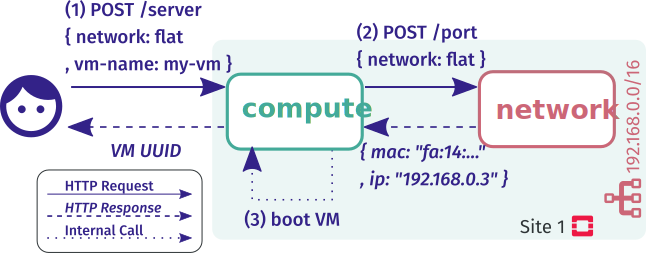
\includegraphics[width=.75\linewidth]{./figs/pdf/network-solo.pdf}
  \caption{Boot of a VM attached to a flat network locally }
  \label{fig:network-solo}
\end{figure}

Now, if we consider two different sites, with \sTwo also having a
physical flat network, but on a different domain (\ie ``10.0.0.0/8'').
%
Therefore a problem may occur if the user wants to use the share
operation such as ``boot a VM on \sOne using the flat network from
\sTwo''.
%
This operation can be expressed in \scl with the following command:
\begin{lstlisting}[numbers=none]
  openstack server create my-vm --network flat \
  --scope { compute: Site1, network: Site2 }
\end{lstlisting}

\begin{figure}[htbp]
  \centering
  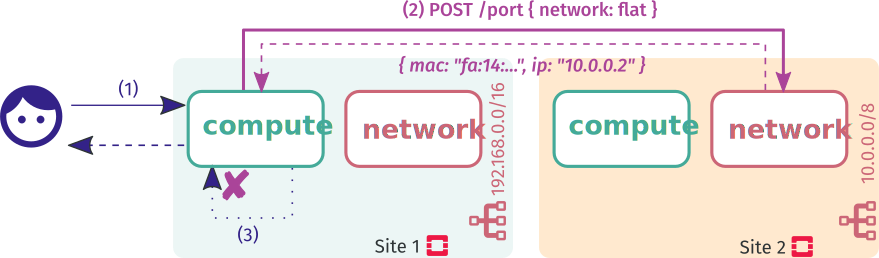
\includegraphics[width=.9\linewidth]{./figs/pdf/network.pdf}
  \caption{Launching a VM with a network, using collaboration}
  \label{fig:network}
\end{figure}

Such an operation makes no sense, as it is presented
in~\autoref{fig:network}.
%
\sTwo returns a port for its physical network (step 2 response) as it
usually would.
%
It includes the IP address ``10.0.0.2'' that is going to be used by
the VM in \sOne (step 3).
%
Unfortunately, \sOne has a different physical network
(``192.168.0.0/16'').
%
Therefore, though this operation is executed successfully, the VM
created with this address becomes unreachable.


Similarly to name bindings in programming languages, we say that
resources have a scope that defines their \emph{visibility}.
%
This scope could be local to one application instance (\eg in our
example, a physical network should only visible by its local site).
%
Or it could be global to all application instances (\eg in OpenStack,
an image is visible by all instances).


Sharing a resource with a local scope such as in
Figure~\ref{fig:network} is a problem.
%
Here, the VM is created with \emph{side effects} that are associated
with this creation.
%
These effects are costly because they uses multiple resources while
being of no use (since the VM will be unreachable).
%
More importantly, it is impossible to define a general rollback
strategy that undo all these side effects.
%
So it is crucial that each resource sharing is validated before its
execution.

A naive approach to identify invalid resource sharing would be to
exhaustively list all correct ones.
%
While it is a pragmatic approach for a specific use case, it does not
offer extensibility and lacks of generality.
%
This approach could work for one given version of an application, but
any changes or additional features would result in invalidating the
aforementioned list.

To avoid such dependencies to one specific application, we propose to
leverage memory access control techniques.
%
In programming, a particular information has a validity in its own
memory context.
%
This information can be used in different contexts as long as there is
a \emph{reference} that enables its access.
%
Sharing and copying this reference into other pointers leads to a
well-known issue called pointers aliasing (\eg dangling pointers).
%
An simple example of a dangling pointer is presented
in~\autoref{fig:dangling-pointer}.
%
A pointer ptr1 references an object by its address in the memory.
%
At some point, a copy of the pointer (ptr2) is made, for example for a
shallow copy of the object.
%
The object goes out of scope, either because it was a local variable
and the function is done, or because a user deletes it.
%
The memory is de-allocated, but ptr2 still points to it.
\begin{figure}[htbp]
  \centering
  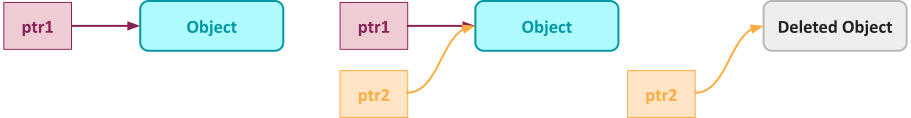
\includegraphics[width=.9\linewidth]{./figs/pdf/dangling-pointers.pdf}
  \caption{Dangling pointer example.}
  \label{fig:dangling-pointer}
\end{figure}

%
Among the solutions that have been proposed to deal with this issue,
the ownership types (\acrshort{OT})~\cite{CPN98,BLS03} has defined the
notion of containment.
%
At coarse-grained the idea is to only allow the owner of the memory
space to access it, preventing references sharing and copying.

We propose to use in the future this concept in \scl to prevent wrong
collaborations.
%
In the network scenario, \sTwo owns a network resource but the user
shares its reference with \sOne.
%
It resembles the dangling pointer problem: the scope of the network
is \sTwo and so cannot be reached by \sOne.
%
The sharing of this resource must be prevented.

Using \acrshort{OT}, it becomes possible to specify the scope of this
resource (\ie a type that defines which \os instances is its owner).
%
This type can be used in a type-checker to prevent any wrong sharing a
priori.
%
The pseudo-code in Figure~\ref{lst:OT} shows the OT annotations
and type-checking of our network scenario.
%
We first define the services (l.~1-4). Then instantiate them with
Compute in \sOne and Network in \sTwo (l.~6-9).
%
Finally, we create a VM on \sOne using a reference to the network from
\sTwo (l.~11-12).
%
Here, the type-checker complains about the ownership of the network.

\begin{figure}[tb]
  \lstset{moredelim=[is][\color{Purple}]{$$}}
  \begin{lstlisting}
class Network$<m>$:  # Network service
  def getFlatNetwork() -> $m/$FlatNetwork: #...
class Compute$<m>$:  # Compute service
  def createVM(network: $m/$FlatNetwork)-> $m/$VM: #...

# Code of the OpenStack CLI for
# > openstack server create --network flat
network: $Site2/$Network = Network$<Site2>$()
compute: $Site1/$Compute = Compute$<Site1>$()

flat_net: $Site2/$FlatNetwork = network.getFlatNetwork()
compute.createVM(flat_net)
#                ^ mismatched types:
#                  `createVM` expects `Site1/FlatNetwork`,
#                  but found `Site2/FlatNetwork`.
  \end{lstlisting}
  \caption{Ownership types {\color{Purple}(in purple)} to prevent invalid collaborations}
  \label{lst:OT}
\end{figure}

The \acrshort{OT} proposal should not need changes in the business
code of the application.
%
However, it requires to type services API in addition to implement a
type-checker.

This ownership types approach should be developed further to help
ensure that sharing of resources will be done in a manner that
prevents non valid sharing.

This approach is a long haul to consider and implement and thus is
considered for the distant future of Cheops.



\chapter{Conclusion} % 3p
%\addcontentsline{toc}{chapter}{Conclusion}


The Edge computing paradigm has shifted the way applications need to
be designed to cope with a hostile environment where disconnections
are the norm rather than the exception.
%
With the need for low latency and robustness against disconnections,
it is difficult to envision using existing applications designed for
the Cloud at the Edge.

To run such an application on such a widely spread infrastructure, it
is crucial to consider scalability as well as locality and tolerance
to faults in the infrastructure.

In this thesis, I have studied how it is possible to avoid creating
new applications specifically for the Edge, but rather use existing,
service-based Cloud applications.


\section*{Summary of the approach}

To deal with the latency and disconnections, the application used need
to be deployed entirely on each Edge location, which allows for a
local-first approach, where the application work autonomously on each
location.
%
Then, to allow for a single coherent system cherished in distributed
systems, for mobility and the usage of the entire infrastructure, it
is mandatory to give the application the ability to be
collaborative-then.
%
To allow for site collaborations, we need to be able to manipulate the
location of request executions.

As Cloud applications can be huge, the solution needs to be generic
and non-intrusive to avoid treating location information in the
business code, so it is necessary to externalize the geo-distribution
concerns outside of the application.
%
Finally, because the Edge infrastructure is highly dynamic (with sites
disconnections and failures) and to allow users to decide the location
of the request execution (\eg for privacy), it is important to give
them the ability to choose it on-demand, dynamically.

The study of the state-of-the-art gave good hints on how to make all
of these requirements happen in a P2P, fully decentralized manner,
though it did not provide an entire solution for all of them.

%
A service-mesh dedicated to the management of the geo-distribution and
collaborations between applications was the solution that fit all the
requirements to put existing Cloud applications at the Edge.
%
To allow this approach, \scl is the DSL that supports the
user-defined, on-demand, fine-grained request descriptions.
%
The modularity of the service-based Cloud applications and the way
their services communicate with each other through REST APIs are the
major elements that helped our approach, by allowing the forwarding of
requests, on top of which different collaborations are possible.


The current version grants three types of collaborations: sharing,
that uses a resource from another site, replication, which allows
users to put identical resources on different sites, and ensures that
they will stay identical from the API point of view, and cross, which
allows resources spanning across different sites.
%
These three collaborations enable the use of resources locally first,
and across sites when needed.
%
They help to lower latency, allows redundancy, fault tolerance, and
along with the users defined requests, they give the users the ability
to choose at fine-grain where their requests will be executed and
which resources to use, which also ensure their privacy, as they can
select what sites they trust.
%
In particular, the replication uses well known algorithms and logic to
ensure consistency and tolerance to fault partition and it allows
users to manipulate whichever replicas is closer/available.

As perspectives to improve this work, I gave hints of possible
extension of collaborations thanks to the genericity of the approach
regarding resources.
%
I also presented the classification of dependencies to ensure the
proper manipulation of linked resources.
%
Finally, for the long haul, I explained how to prevent non-valid
sharings through the use of ownership types.
%

\section*{Overview of the parts and chapters}

This manuscript was built as this following description:
\begin{description}
\item[The introduction] asserts the problematic of this manuscript. To
  be more descriptive, the goal is mainly to answer the question: is
  it possible to bring Cloud applications to the Edge? And with even
  more specifics, can it be applied to Cloud infrastructures
  management applications, and could we use a service-mesh approach to
  do it?
\item [\autoref{p:context}] explains the context of the manuscript.
  \begin{description}
  \item [\autoref{chap:cloud}] described the Cloud overall to give the
    reader a context of what the Cloud is. It gave a view of how Cloud
    applications function and how to manage the Cloud infrastructures to
    give a basis to understand the approach presented in this thesis.
  \item[\autoref{chap:edge}] presented the Edge and its challenges to
    explain on which expectations we were going to build our
    approach. We then defined the principles which we think are
    necessary to follow when developing or adapting an application in
    the context of the Edge.
  \item[\autoref{chap:cloud-app-to-edge}] described in more details
    how it is possible to adapt a Cloud application for the Edge and
    why the required collaborations are not good solutions for me as
    they imply really intrusive changes.
  \end{description}
\item [\autoref{p:soa}] depicts the State-of-the-art regarding the
  management of applications at the Edge, whether they were natively
  built for it or brought from the Cloud.
  \begin{description}
  \item[\autoref{chap:comparison} \textnormal{and}
    \autoref{chap:soa-conclusion}] serve as introduction and conclusion
    for the State of the Art. The first present how we evaluated the
    literature and the latter present the overall comparison.
  \item[\autoref{chap:soa-edge-infra}] presented six approaches to
    manage the infrastructure and more importantly, applications on top
    of it. It also presented in \autoref{chap:soa-SM} to of the most
    known service meshes to better understand how they function and how
    they behave regarding our requirements.
  \item[\autoref{chap:soa-dev-edge-app}] showed two different approaches
    to develop an Edge-native application or adapt an existing one with
    intrusive changes.
  \end{description}
\item [\autoref{part:cheops}] introduces my approach to bring Cloud
  applications to the Edge using a service mesh like aproach.
  \begin{description}
\item[\autoref{chap:overview}] explained our own theoretical approach
  to respond to the expectation we presented in
  \autoref{sec:principles}.
\item[\autoref{chap:cheops}] presented in more detail the PoC we
  develop to correspond to the aforementioned approach, in particular
  the way the replication is implemented and how it was tested.
\end{description}
\item[The conclusion chapters] above presented discussions about our
  approach, its limitations and different perspectives to improve it.
\end{description}
